% paper.tex -- compile with:  pdflatex paper.tex  (twice, for references)
% The four figures it includes are produced by `python figures.py`.
\documentclass[11pt,a4paper]{article}

\usepackage[T1]{fontenc}
\usepackage[utf8]{inputenc}
\usepackage{lmodern}
\usepackage[margin=2.6cm]{geometry}
\usepackage{amsmath,amssymb}
\usepackage{booktabs}
\usepackage{graphicx}
\usepackage{xcolor}
\usepackage{listings}
\usepackage[hidelinks]{hyperref}

\newcommand{\code}[1]{\texttt{\detokenize{#1}}}
\newcommand{\pf}[1]{\textit{#1}}

\lstset{
  basicstyle=\ttfamily\small,
  keywordstyle=\color{black!70},
  commentstyle=\itshape\color{black!55},
  columns=fullflexible,
  frame=leftline,
  framesep=6pt,
  xleftmargin=10pt,
  breaklines=true,
  language=Python,
  showstringspaces=false,
}

\title{An executable Collins \& Stabler (2016):\\
a self-validating derivation driver for minimalist syntax}
\author{Norberto Moreno-Quibén\\
  University of Alcalá\\
  \texttt{norbmor@gmail.com}}
\date{}

\begin{document}
\maketitle

\begin{abstract}
\noindent
Collins \& Stabler (2016) give an axiomatization of minimalist syntax:
forty-four definitions, five Chain-based variants and fourteen theorems,
stated precisely enough that one can ask whether a given sequence of
operations is a derivation. We transcribe it into executable Python and wrap
it in a driver that refuses to take a step the definitions do not license, so
that a derivation object is a certificate rather than a transcript. Seventeen
derivations validate against D14/D38 and theorems T5--T10. The
implementation reproduces the paper's central argument mechanically: with the
structural notion of finality of D40, remnant movement inside one phase is
spelled out correctly, but under the plug-back-in model of Transfer the
paper's example (21) is pronounced \pf{how likely John to win you think that
John is}, and that derivation still converges. An implementation of the
section 12 alternative pronounces it correctly. We also report three things
the paper does not: Theorem 4 (the token/Chain correspondence) fails on
exhaustively enumerated fragments from three Merge nodes on, under both
readings of its garbled locality condition that we tested; the section 12 sketch works under
one reading of ``W minus those already transferred'' and makes
successive-cyclic movement underivable under the other; and, with the
unordered trigger features the paper assumes, adding selection still admits
the $[_{\mathrm{TP}}\ \mathrm{vP}\ [_{\mathrm{T'}}\ \mathrm{T}\ \mathrm{DP}]]$
orders that section 7 says something else must exclude.
\end{abstract}

\section{What we set out to build}

Collins \& Stabler (2016) is unusual among formalizations of minimalism in
that it is complete enough to be mechanical. It defines lexical items,
workspaces, Select, Merge, occurrences, derivations, labels, Transfer and
convergence, and it states theorems about them. Our question was whether the
axiomatization survives being taken at its word: if one implements exactly
what the definitions say, do the paper's derivations go through, do its
theorems hold, and what happens where the prose has to do work the
definitions do not?

The deliverable is a \emph{self-validating derivation driver}. Each method
call constructs the next stage and asserts that the previous stage derives it
by one of the clauses of D14/D38 before accepting it:

\begin{lstlisting}
from derivations import LEX
from cs2016 import Derivation, labelled_bracket

d = Derivation(LEX, [LEX.token("fall", 1), LEX.token("John", 2),
                     LEX.token("T_V", 3), LEX.token("Comp", 4)])
d.select("fall", 1).select("John", 2).merge_roots()
d.select_and_merge("T_V", 3)
d.internal_merge(LEX.token("John", 2))
d.select_and_merge("Comp", 4)
print(labelled_bracket(d.root))
# [CP Comp4 [TP John2 [T' T_V3 [VP fall1 <John2>]]]]
d.transfer()          # D38(a): Transfer(CP, CP)
d.check()
\end{lstlisting}

\noindent
An illegal move raises an error naming the definition it violates. Selecting
outside the lexical array reports D12, merging a trigger-less selector
reports D27, and transferring a phase that contains a phase with an
untransferred complement reports D38.

Three commitments follow from ``transcription, not re-engineering''. Every
public name is tagged with the number of the definition or theorem it
implements. Nothing is enforced that the paper does not state. And where the
paper leaves a choice open, the code makes one and marks it
\code{# STIPULATION}.

\section{What the transcription buys}

\paragraph{Definitions become testable one at a time.} The test suite has 55
checks: one per definition cluster, theorem, paper example or finding. A
second suite has 21 checks over added constructions. Occurrences are paths
(D16--D22), so T1--T3 can be checked on every object built.

\paragraph{Theorems become checkable everywhere.} Select shrinks the lexical
array and each Merge checks one trigger feature, so the state graph from a
lexical array is finite and acyclic. Section~\ref{sec:selection} walks all
4{,}072 reachable stages of one array and finds T5, T6, T8 and T9 holding
throughout.

\paragraph{Two results fall out rather than being stipulated.} The PIC is
Theorem 14 and follows from a typing fact. Cyclic-Transfer replaces the
complement by a pair that D37 declines to call a syntactic object, and Merge
is defined only on syntactic objects. Successive cyclicity is forced in the
same indirect way. Without the step to the matrix v* edge, \pf{who} is
trapped inside the complement transferred at that phase
(Figure~\ref{fig:wh}).

\section{Coverage}

Table~\ref{tab:coverage} lists what the driver validates. Every derivation
satisfies D14/D38, D15, T5, T6, T7, T8 at Select and Merge, T9 and T10. PF
and the convergence verdicts are computed by D41--D43 at report time.

\begin{table}[htbp]
\centering
\footnotesize
\setlength{\tabcolsep}{4pt}
\begin{tabular}{llrrlcc}
\toprule
derivation & source & steps & C-T & PF & CI & SM \\
\midrule
\code{external_merge_6}            & (6)/(8), D13 &  5 & 0 & --- & --- & --- \\
\code{internal_merge_7}            & (7), D13   &  4 & 0 & --- & --- & --- \\
\code{two_trigger_features_15}     & (15)       &  4 & 0 & --- & --- & --- \\
\code{vp_see_chris}                & (16)/(17)  &  3 & 0 & --- & --- & --- \\
\code{john_fell}                   & (18)       &  9 & 0 & \pf{John fell} & yes & yes \\
\code{remnant_movement}            & (19)/(20)  & 16 & 0 & \pf{how likely to win John is} & yes & yes \\
\code{remnant_across_phases}       & (21)       & 31 & 2 & \pf{how likely John to win \dots\ John is} & yes & yes \\
\code{crashing}                    & D42        & 14 & 1 & \pf{John see Chris} & \textbf{no} & yes \\
\midrule
\code{john_sees_chris}             & added      & 14 & 1 & \pf{John see Chris} & yes & yes \\
\code{successive_cyclic_wh}        & added      & 31 & 3 & \pf{who you think John will see} & yes & yes \\
\code{john_seems_to_win}           & added      & 13 & 0 & \pf{John seem to win} & yes & yes \\
\code{you_wonder_who_john_will_see}& added      & 29 & 3 & \pf{you wonder who John will see} & yes & yes \\
\code{john_gives_mary_flowers}     & added      & 16 & 1 & \pf{John Mary give flowers} & yes & yes \\
\code{mary_praises_john}           & added      & 14 & 1 & \pf{Mary praise John} & yes & yes \\
\code{mary_not_praise_john}        & added      & 16 & 1 & \pf{Mary not praise John} & yes & yes \\
\code{sue_thinks_john_fell}        & added      & 22 & 2 & \pf{Sue think John fell} & yes & yes \\
\code{who_does_sue_think_fell}     & added      & 25 & 2 & \pf{who Sue think fell} & yes & yes \\
\bottomrule
\end{tabular}
\caption{The derivations the driver validates. ``steps'' counts Select,
Merge and Transfer operations; ``C-T'' counts Cyclic-Transfer steps. The
first four have no Transfer step, so the convergence definitions, which
inspect $W_n = \{\langle \mathrm{PHON},\mathrm{SEM}\rangle\}$, do not apply.
The first two use D13 (untriggered) Merge, as section 3 of the paper does.
\code{remnant_across_phases} converges although its PF is wrong
(Section~\ref{sec:remnant}).}
\label{tab:coverage}
\end{table}

\section{Remnant movement and the plug-back-in model}
\label{sec:remnant}

The 2016 definition of finality is structural (D40): $A \in \{A,B\}$ is
non-final in a phase iff some $C$ in the phase has $A$ as a member and
contains $\{A,B\}$. In (20d) the TP has \pf{John} as a member and contains
$\{\mathit{John},\{\mathit{to},\mathit{win}\}\}$, so \pf{John} is non-final
in \emph{both} copies of the moved DegP. One Transfer at (20d) gives
\pf{how likely to win John is} (Figure~\ref{fig:remnant}a). If Transfer
applies at (20c) instead, before the remnant moves, the DegP is inside the
transferred TP and cannot move (T14). Both facts are tested.

The paper then argues that this solution does not survive a second phase.
The driver confirms this. In (21) the embedded TP has been replaced by its
interface pair before the matrix CP is spelled out, so at the matrix level
nothing contains $\{\mathit{John},\{\mathit{to},\mathit{win}\}\}$ and has
\pf{John} as a member. \pf{John} is final again and is pronounced twice:
\pf{how likely John to win you think that John is}
(Figure~\ref{fig:remnant}b). Two further observations are not in the paper:

\begin{itemize}
\item \emph{The failure is invisible to convergence.} Every step is licensed
and the derivation converges at both interfaces (D42--D44), because those
definitions inspect features, not the relation between PF and structure.
\item \emph{It also arises in one phase.} D38 licenses Cyclic-Transfer at
(20d) followed by Transfer(SO,SO). In that derivation the TP is plugged back
in before the final spell-out, and the one-phase example comes out as
\pf{how likely John to win John is}.
\end{itemize}

\begin{figure}[htbp]
  \centering
  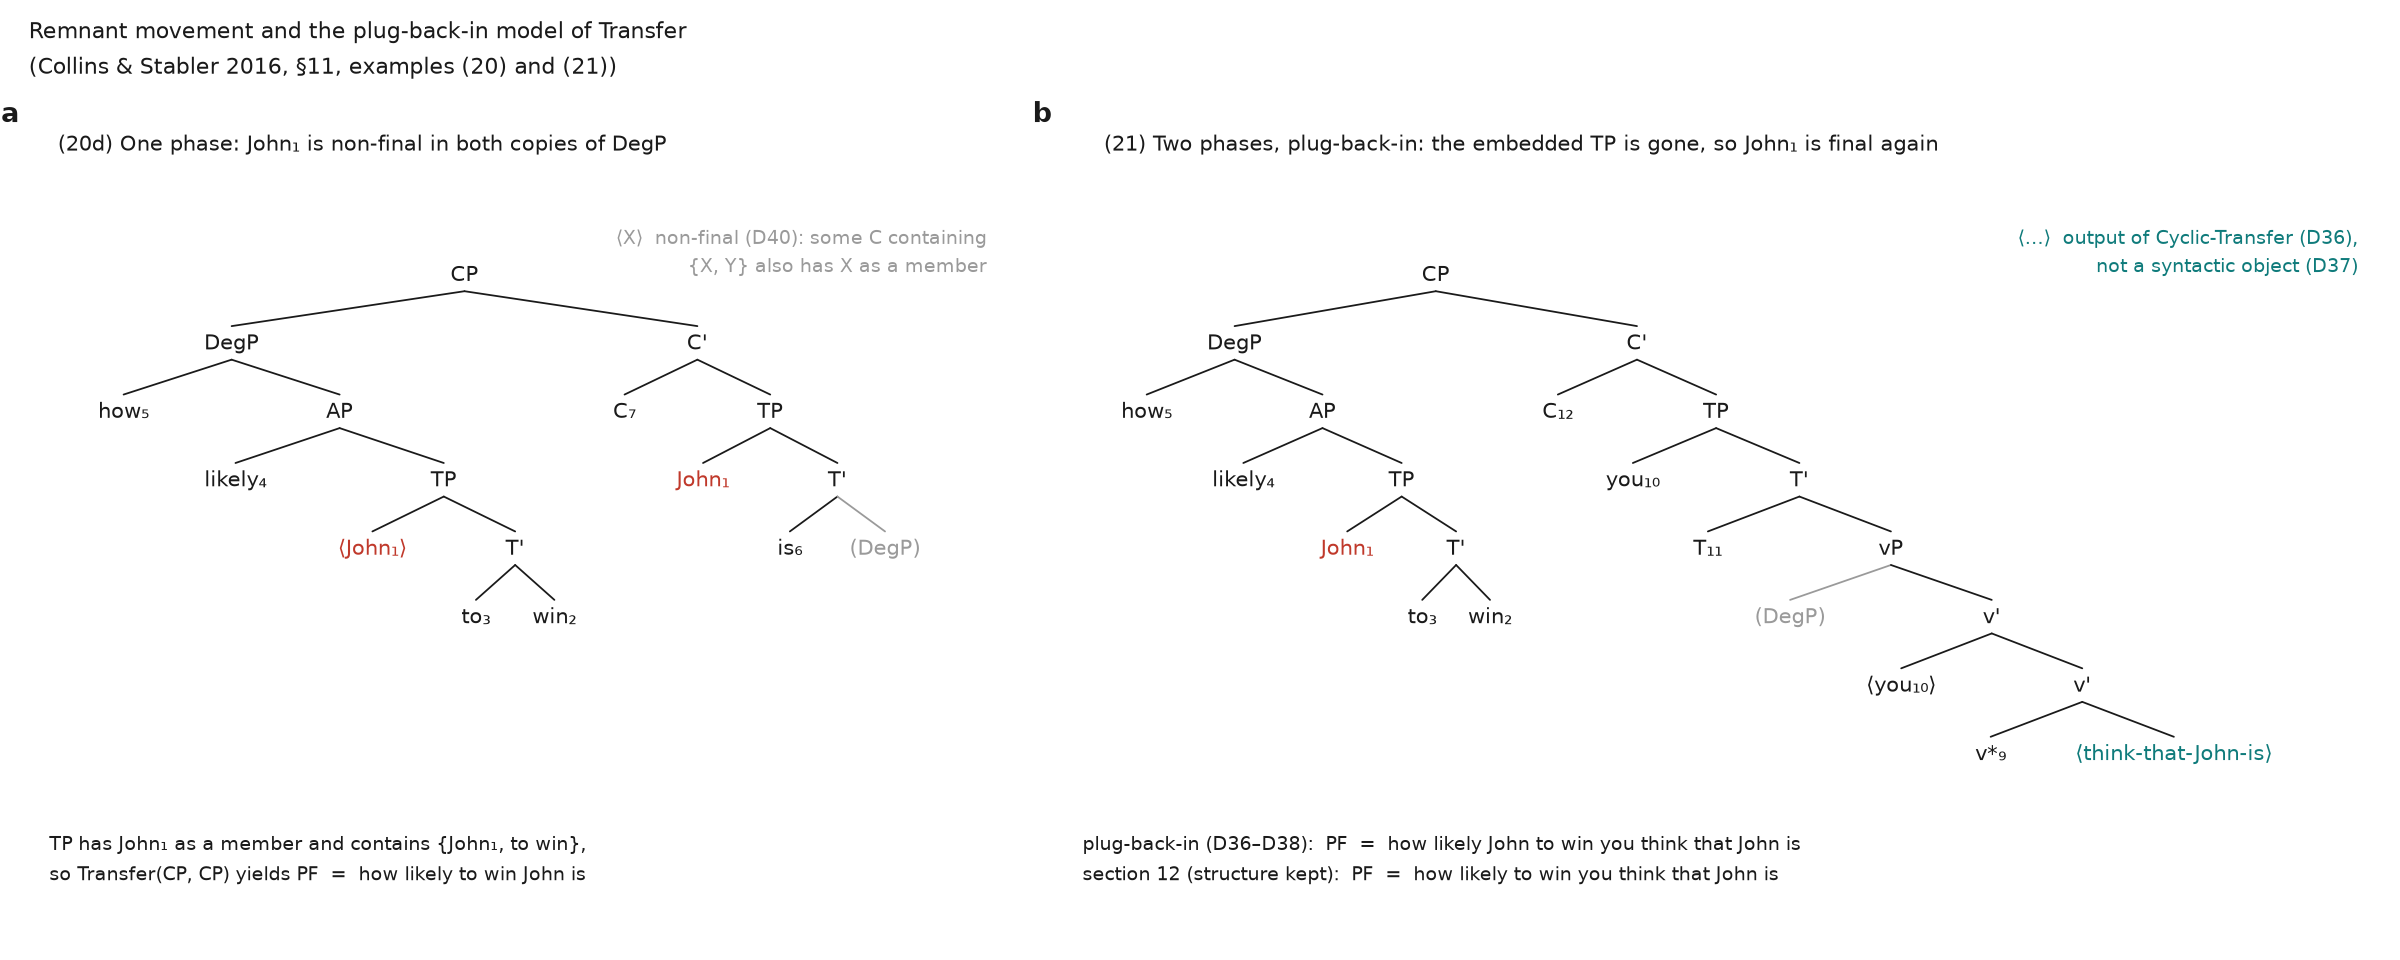
\includegraphics[width=\linewidth]{remnant_derivation.png}
  \caption{Remnant movement (C\&S 2016, (20) and (21)). Both panels are
  read off validated derivation objects: node labels from D28, daughter
  order from D41b, angle brackets from D40. \textbf{(a)} In one phase,
  \pf{John}$_1$ is non-final in both copies of the DegP. \textbf{(b)} Across
  two phases under the plug-back-in model, the embedded TP has been replaced
  by a transferred pair, and \pf{John}$_1$ in the moved DegP is final.}
  \label{fig:remnant}
\end{figure}

\section{The section 12 alternative}

Section 12 sketches an NTC-respecting Transfer. Transfer extends two
functions PF and LF instead of altering the tree, the transferred objects are
their domain, and ``the accessible parts of workspace W are given by W minus
those already transferred''. The formal version is in an appendix that was
not published. We implemented the sketch (\code{NTCDerivation}). It does what
the paper says: T8 holds at every Transfer step; D7 suffices, since no
transferred pair ever enters the workspace; the PIC holds by an accessibility
stipulation; and (21) comes out as \pf{how likely to win you think that John
is}. On every derivation in which nothing moves out of a moved phrase, the
two models give the same PF and LF (Table~\ref{tab:regimes}).

\begin{table}[htbp]
\centering
\footnotesize
\begin{tabular}{lll}
\toprule
derivation & plug-back-in & section 12, object reading \\
\midrule
\code{remnant_movement}      & \pf{how likely to win John is} & \pf{how likely to win John is} \\
\code{remnant_across_phases} & \pf{how likely John to win you think\dots} & not derivable \\
\code{successive_cyclic_wh}  & \pf{who you think John will see} & not derivable \\
\code{you_wonder_who_john_will_see} & \pf{you wonder who John will see} & not derivable \\
\code{who_does_sue_think_fell} & \pf{who Sue think fell} & not derivable \\
\bottomrule
\end{tabular}
\caption{The rows of \code{transfer_regime_comparison.csv} where the
regimes differ. The section 12 occurrence reading gives the correct string
on all of them. Every other derivation is identical under all three
regimes.}
\label{tab:regimes}
\end{table}

\paragraph{Under-determined: what is subtracted.} ``W minus those already
transferred'' can be read per occurrence (an occurrence is inaccessible iff
its path passes through a transferred object) or per object (an object is
inaccessible iff it is contained in a transferred object). They come apart
whenever something has moved to a phase edge. The edge copy is accessible,
but the same object also occurs inside the transferred complement. Under the
object reading, every derivation in which something moves on from a phase
edge is underivable: successive-cyclic wh-movement, the embedded question
(whose \pf{who} leaves the embedded v* edge), and (21), the example section
12 was introduced to rescue.

\paragraph{Under-determined: the stage.} D10 makes a stage $\langle
\mathrm{LA}, W\rangle$. Section 12 moves Transfer's effect into PF and LF,
which the stage does not contain. So a section 12 Transfer step repeats the
previous stage, which no clause of D38 licenses, and D42--D44, which require
$W_n = \{\langle\mathrm{PHON},\mathrm{SEM}\rangle\}$, do not apply. The
repair is to restate the stage as $\langle \mathrm{LA}, W, \mathrm{PF},
\mathrm{LF}\rangle$, and it shows that section 12 revises the definition of
a derivation, not only that of Transfer.

\section{Theorem 4: tokens versus Chains}

Section 5 defines a Chain-based system without indices, in which a set formed
by internal Merge carries the path to the moved item (D7$'$,
D13$'$--D16$'$). Theorem 4 asserts a one-to-one, onto, structure-preserving
correspondence between token-based objects up to renumbering (excluding
merges of renumberings) and Chain-based objects. We enumerated both sets for
the lexicon $\{\mathit{John},\mathit{see}\}$ up to five Merge nodes. Each
token object was mapped to the Chain object with the same structure and the
image of the same path (Table~\ref{tab:t4}).

\begin{table}[htbp]
\centering
\footnotesize
\begin{tabular}{lrrrrrc}
\toprule
D14$'$(c) & size & tokens & Chains & no image & $>1$ image & bijection \\
\midrule
our reading & 2 &   7 &    7 &   0 &   0 & yes \\
our reading & 3 &  25 &   23 &   2 &   0 & no \\
our reading & 5 & 703 &  437 & 272 &   6 & no \\
dropped     & 2 &   7 &    7 &   0 &   0 & yes \\
dropped     & 3 &  25 &   27 &   0 &   2 & no \\
dropped     & 5 & 703 & 1097 &   0 & 224 & no \\
\bottomrule
\end{tabular}
\caption{Token classes against Chain-based objects, by maximal number of
Merge nodes (\code{theorem4_check.csv}). Every Chain object has a token
preimage. The failures are token classes with no image, or with several.}
\label{tab:t4}
\end{table}

The locality condition D14$'$(c) is misprinted. As written it quantifies over
every node of the path above $B$, including $B$'s mother, so it would block
every internal Merge, the paper's own (7$'$) included. We read it as
excluding paths that pass a higher occurrence of $B$. Under that reading, the
token system derives $\{\mathit{see}_2,\{\mathit{see}_3,\{\mathit{John}_1,
\mathit{see}_2\}\}\}$, in which a lower token moves across a higher token of
the same item, and the Chain system cannot, because there the two
\pf{see}s are one object and (c) selects the higher. Remnant configurations
fail in the other direction. When an item occurs inside both copies of a
moved phrase, neither occurrence c-commands the other, and one token object
has two Chain counterparts. Dropping (c) instead lets the Chain system record
\emph{which} occurrence of an already-moved item is re-merged, a distinction
the paper notes the token system never makes. Under both readings we tested,
the natural correspondence fails from three Merge nodes on. The
paper's proof is unpublished, so we cannot exclude a different
correspondence. But it would have to disregard the paths, which are the
point of the Chain-based system.

\section{Selection and unordered triggers}
\label{sec:selection}

Triggered Merge (D27) checks only that Triggers(A) is non-empty and
Triggers(B) is empty, never that the trigger matches B. Adding the match and
enumerating every complete derivation (D15) from
$\{\mathit{see}_1, \mathit{Chris}_2, v^*_3, \mathit{John}_4, T_5,
\mathit{Comp}_6\}$ gives Table~\ref{tab:selection}.

\begin{table}[htbp]
\centering
\footnotesize
\begin{tabular}{lrrrrc}
\toprule
Merge rule & derivations & objects & stages & PF strings & T5, T6, T8, T9 \\
\midrule
D27 Triggered Merge                &  6{,}267{,}280 & 648 & 4{,}072 & 6 & all hold \\
\quad + selection, ranked          &      55{,}968 &  12 &    280  & 6 & all hold \\
\quad + selection, ranked, EPP needs D & 27{,}984 &   6 &    178  & 4 & all hold \\
\quad + selection, unranked        &     171{,}424 &  24 &    448  & 6 & all hold \\
\quad + selection, unranked, EPP needs D & 85{,}712 & 12 &   304  & 4 & all hold \\
\bottomrule
\end{tabular}
\caption{Every complete derivation the array admits under each rule.}
\label{tab:selection}
\end{table}

Three points. First, the general theorems hold under every rule: they follow
from the stage/workspace format of D10 and D14, not from what licenses a
Merge. Second, D26 leaves open which trigger feature a Merge checks, and
under D27 alone the choice is inert: only the number of remaining triggers
matters, and the ranked and unranked policies give identical derivations.
Third, once selection is added the choice matters, and the paper assumes
trigger features are \emph{unordered}. It then asks what excludes
$[_{\mathrm{TP}}\ \mathrm{vP}\ [_{\mathrm{T'}}\ \mathrm{T}\ \mathrm{DP}]]$
and answers that internal Merge of the DP into that position would violate
the NTC. For an externally merged DP nothing does. Unranked selection admits
twice as many objects as ranked selection. Each of the twelve extra objects
has a head whose EPP took a DP as its complement: four are the paper's T
configuration, and eight are the same configuration on v*.

\section{Smaller stipulations}

\textbf{D38 and the lexical array.} The derive-by-Transfer clause of D38 says
nothing about $\mathrm{LA}_{i+1}$; read literally, Transfer could change the
lexical array arbitrarily. We require it to be unchanged.

\textbf{``Replacing A'' in D36} is read positionally: the complement
occurrence is replaced. A phase-head complement with a second occurrence does
not arise in our derivations.

\textbf{Phasehood is enumerated (D35).} \code{is_strong_phase} checks
maximality and a Comp or v* label, which is what D35 says. This is the one
place where the category inventory is hard-coded. The negated clause of
Figure~\ref{fig:neg} adds a category (Neg) at the cost of one selection
feature, and D35 correctly leaves it transparent.

\begin{figure}[htbp]
  \centering
  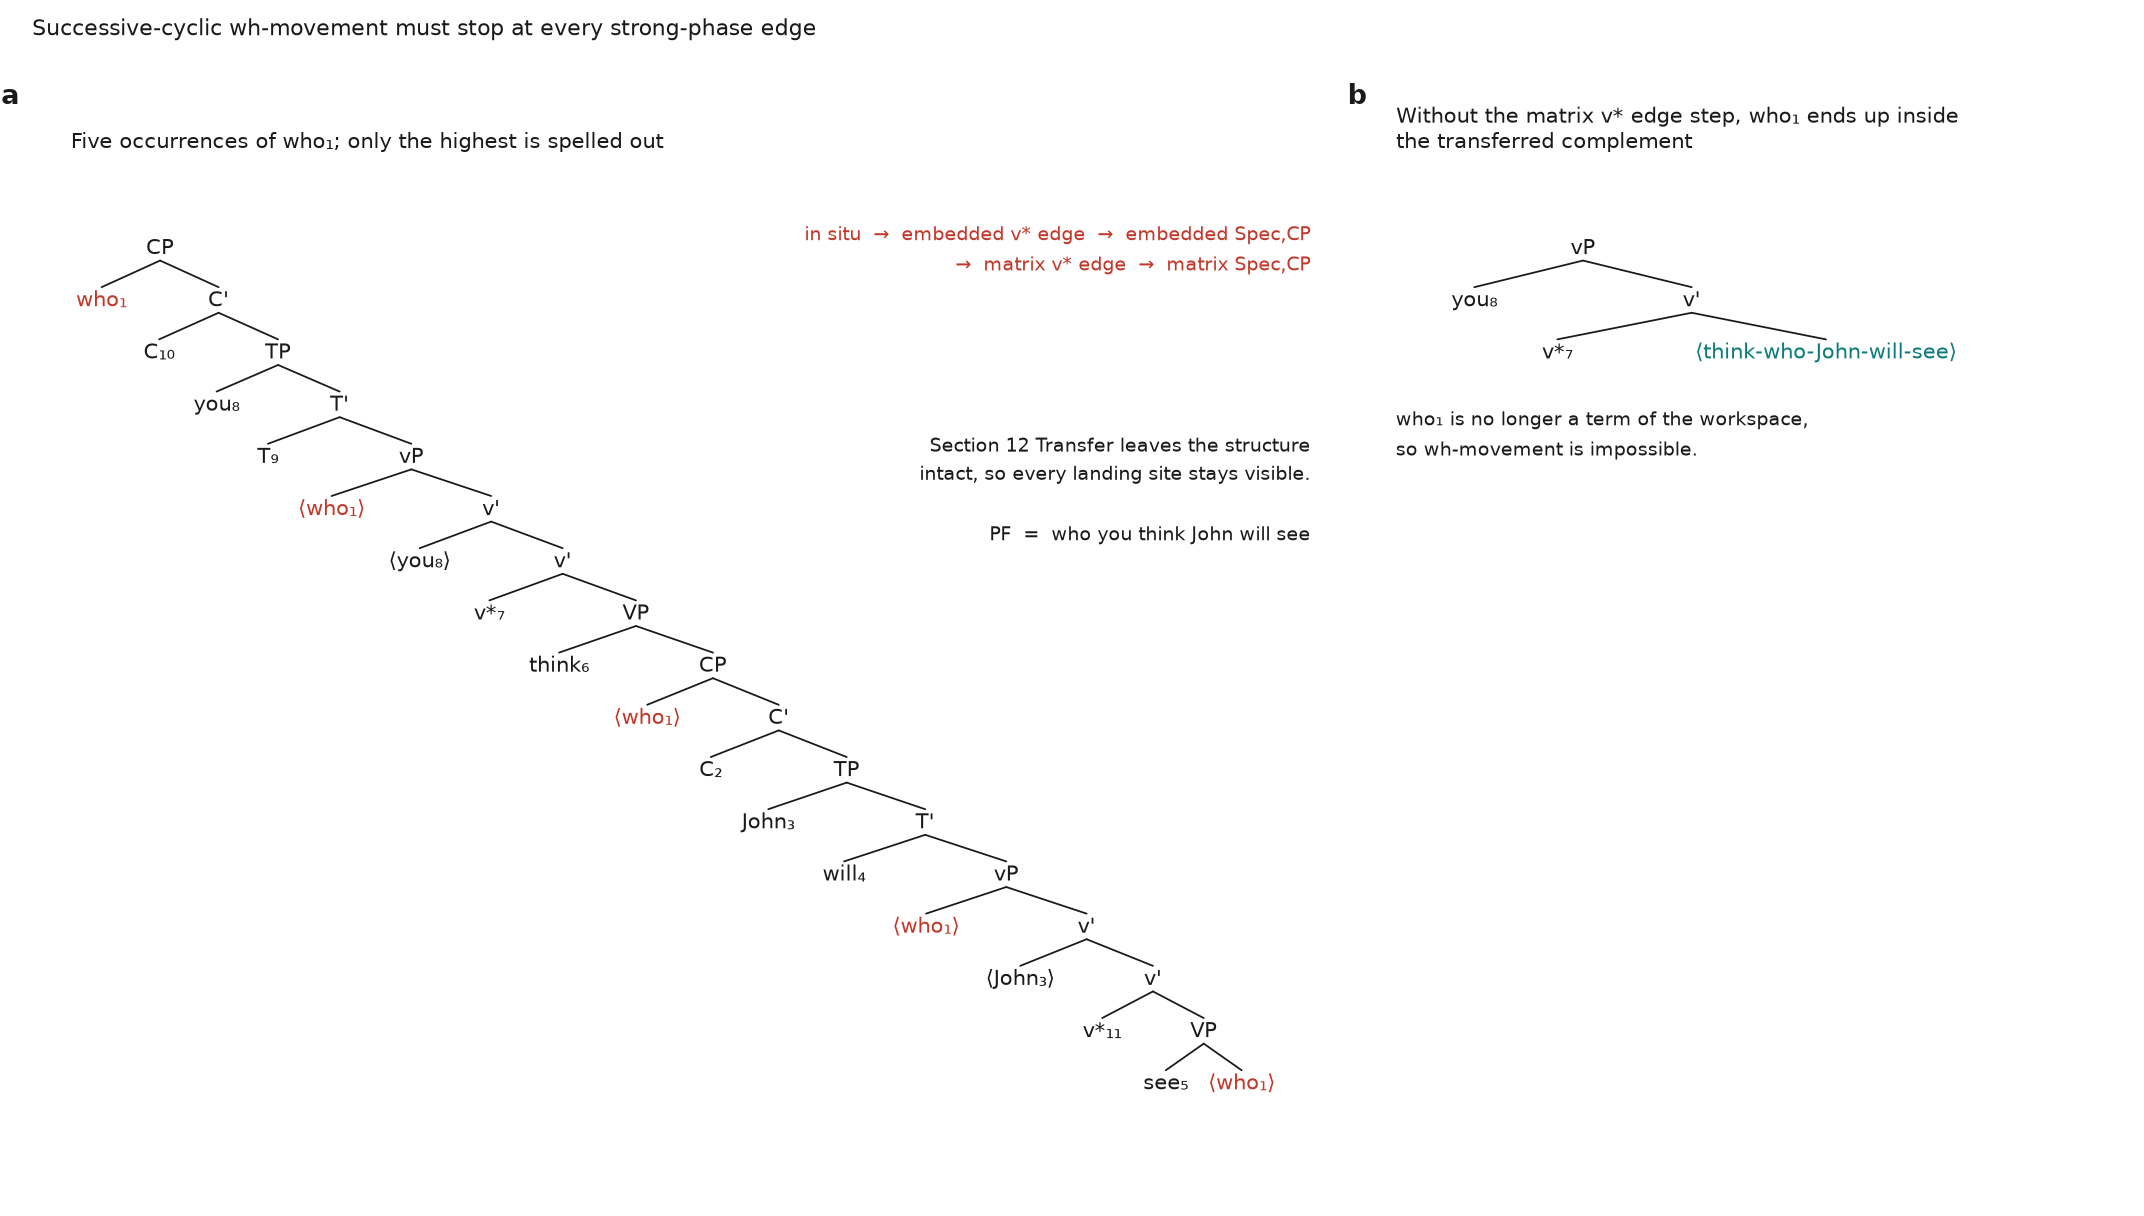
\includegraphics[width=\linewidth]{successive_cyclic_wh.png}
  \caption{Successive cyclicity is forced, not stipulated. \textbf{(a)} The
  five occurrences of \pf{who}$_1$, drawn under the section 12 Transfer,
  which never modifies the workspace. \pf{John}$_3$ is the external argument
  of \pf{see}: it is merged in the embedded Spec,vP and raises to Spec,TP of
  \pf{will}, and \pf{who}$_1$ must pass through the embedded v* edge before
  that phase's VP is transferred. \textbf{(b)} Without the step to the
  matrix v* edge, \pf{who}$_1$ is inside the complement transferred at that
  phase and the final movement is refused (T14).}
  \label{fig:wh}
\end{figure}

\begin{figure}[htbp]
  \centering
  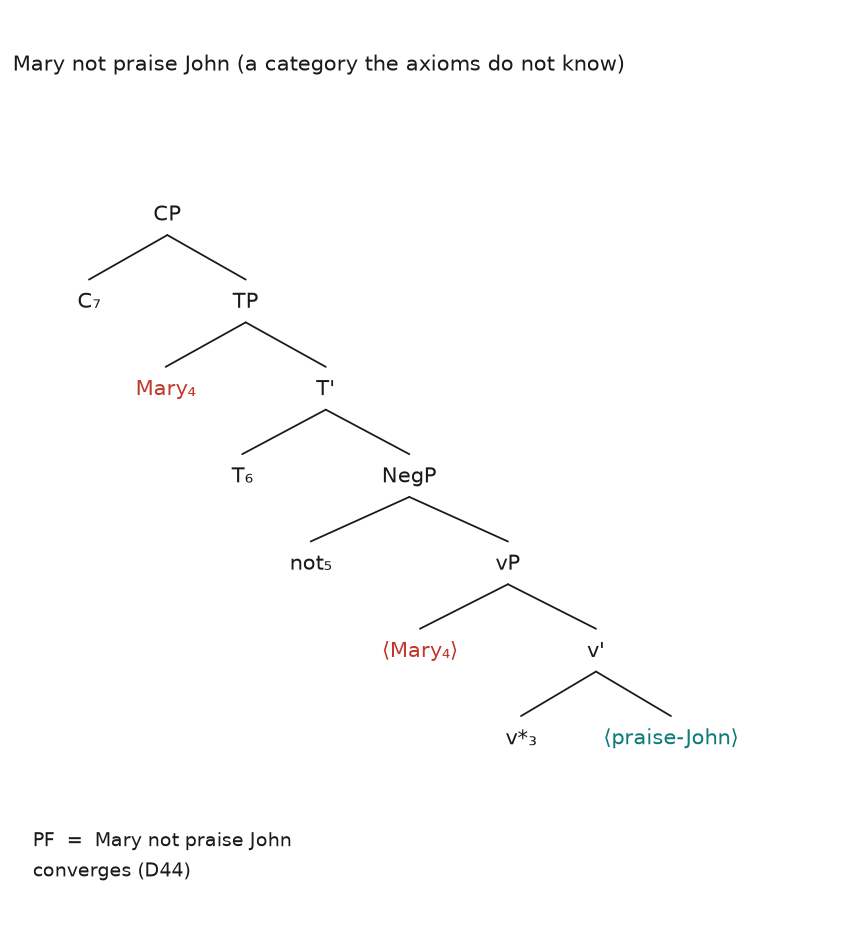
\includegraphics[width=0.66\linewidth]{mary_not_praise_john.png}
  \caption{A category the axioms do not know. Adding Neg costs three lexical
  items and no change to any definition; the chunk transferred at the v*
  phase is identical to the affirmative one. No head movement is formalized,
  so D41b spells the terminals out in Specifier-Head-Complement order.}
  \label{fig:neg}
\end{figure}

\begin{figure}[htbp]
  \centering
  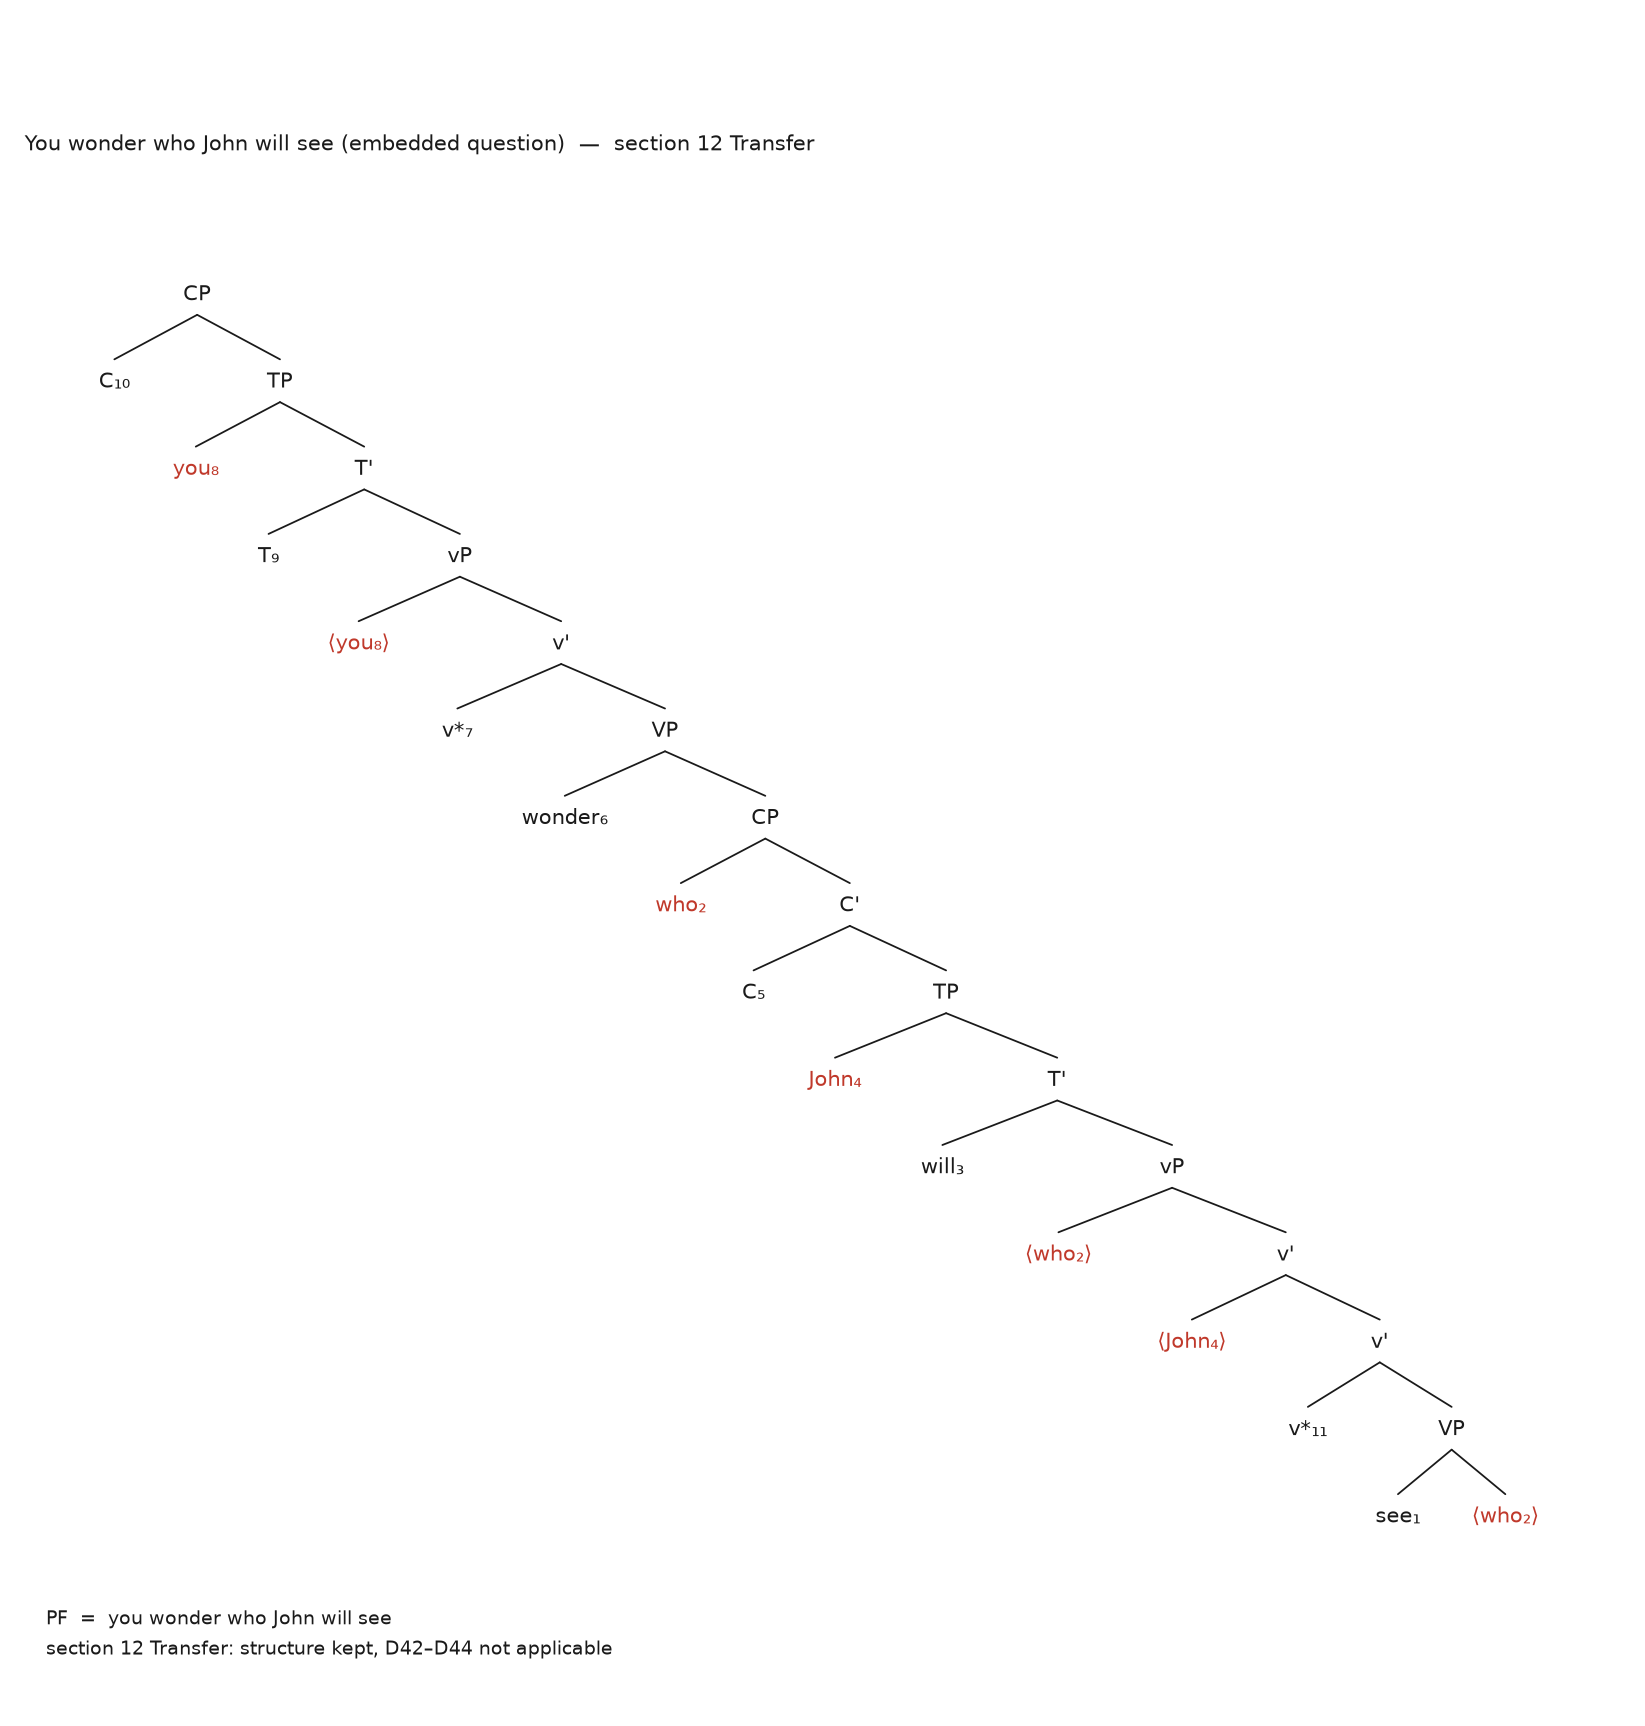
\includegraphics[width=0.66\linewidth]{you_wonder_who_john_will_see.png}
  \caption{An embedded question (added). \pf{who}$_2$ moves through the
  embedded v* edge to the embedded Spec,CP, its only final occurrence (D40),
  and is pronounced inside the chunk spelled out at the matrix v* phase.
  \pf{John}$_4$, the external argument of \pf{see}, is merged in Spec,vP and
  raises to Spec,TP. Drawn under the section 12 Transfer, so the embedded
  structure is not folded into transferred chunks.}
  \label{fig:wonder}
\end{figure}

\section{What is absent: Agree and head movement}

There is no Agree anywhere in the axiomatization. TransferLF (D39) keeps the
whole Sem set of every token, so the crashing derivation (D42) requires a
lexical item that is uninterpretable by stipulation. There is no head
movement either, which is why \pf{John Mary give flowers} and \pf{Mary not
praise John} come out in Specifier-Head-Complement order with no auxiliary.
Both are predictions of the axiomatization as stated, and we document them
rather than working around them.

\section{Reproducibility}

The implementation is standard-library Python; only the figure script needs
matplotlib.

\begin{lstlisting}[language=bash]
python test_cs2016.py     # 55 checks
python test_sentences.py  # 21 checks
python derivations.py     # -> derivation_report.txt
python sentences.py       # -> sentence_report.txt
python tables.py          # the three CSV tables
python figures.py         # the four figures used here
python figures.py --all   # a tree for every derivation
\end{lstlisting}

\noindent
The trace files are byte-reproducible under any hash seed, and the figures
are drawn from validated derivation objects, so a figure cannot show a
structure the axioms did not build.

\section{Conclusion}

Collins \& Stabler's axiomatization survives being taken at its word. The
paper's examples derive, its general theorems hold on every reachable stage
of the arrays we explored, and the PIC and successive cyclicity emerge from
the definitions. The implementation reproduces the paper's own case against
the plug-back-in model exactly as the paper states it, and adds that the bad
derivation converges. Where the system is under-determined, the gaps are
concentrated in the parts the paper marks as sketches or leaves to an
appendix: the section 12 alternative, which works under one reading of
accessibility and not the other, and Theorem 4, whose locality condition is
misprinted and whose natural correspondence fails on small fragments under
both readings we tested.

\begin{thebibliography}{9}
\bibitem{cs2016}
Collins, Chris \& Edward Stabler (2016).
A Formalization of Minimalist Syntax.
\textit{Syntax} 19(1): 43--78. DOI 10.1111/synt.12117.

\bibitem{chomsky2000}
Chomsky, Noam (2000).
Minimalist inquiries: the framework.
In R. Martin, D. Michaels \& J. Uriagereka (eds.),
\textit{Step by Step}. Cambridge, MA: MIT Press, 89--155.

\bibitem{chomsky2004}
Chomsky, Noam (2004).
Beyond explanatory adequacy.
In A. Belletti (ed.), \textit{Structures and Beyond}.
Oxford: Oxford University Press, 104--131.
\end{thebibliography}

\end{document}
